\subsection{UC29 - Modifica suddivisione}
\begin{figure}[H]
  \centering
  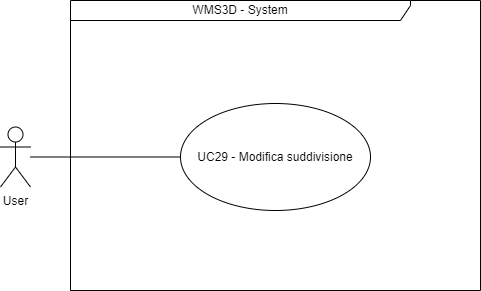
\includegraphics[width=0.6\textwidth]{UC_diagrams_28-32/UC29_sys.drawio.png}
   \caption{Diagramma UML UC29 - Modifica suddivisione}
\end{figure}
\begin{figure}[H]
  \centering
  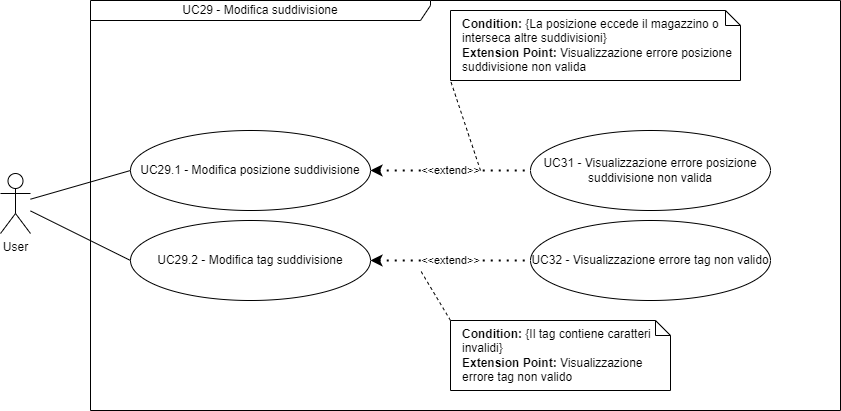
\includegraphics[width=0.9\textwidth]{UC_diagrams_28-32/UC29.drawio.png}
   \caption{Diagramma UML in dettaglio UC29 - Modifica suddivisione}
\end{figure}
\begin{itemize}
    \item \textbf{Attori:} User.
    \item \textbf{Pre-condizione:} L'utente ha selezionato una suddivisione del magazzino precedentemente creata [UC28] da modificare.
    \item \textbf{Post-condizione:} L'utente ha modificato correttamente una nuova suddivisione.
    \item \textbf{Scenario Principale:} L'utente modifica la posizione [UC29.1] e/o il tag [UC29.2] della suddivisione selezionata.
    \item \textbf{Generalizzazioni:} -
    \item \textbf{Estensioni:} -
\end{itemize}

\paragraph{UC29.1 - Modifica posizione suddivisione}
\begin{itemize}
    \item \textbf{Attori:} User.
    \item \textbf{Pre-condizione:} L'utente ha selezionato una suddivisione del magazzino precedentemente creata [UC28] da modificare.
    \item \textbf{Post-condizione:} L'utente ha modificato la posizione della suddivisione.
    \item \textbf{Scenario Principale:} L'utente sceglie una nuova posizione per la suddivisione all'interno della planimetria.
    \item \textbf{Generalizzazioni:} -
    \item \textbf{Estensioni:} È presente una estensione:
        \begin{itemize}
            \item UC31 - Visualizzazione errore posizione suddivisione non valida.
        \end{itemize}
\end{itemize}

\paragraph{UC29.2 - Modifica tag suddivisione}
\begin{itemize}
    \item \textbf{Attori:} User.
    \item \textbf{Pre-condizione:}  L'utente ha selezionato una suddivisione del magazzino precedentemente creata [UC28] da modificare.
    \item \textbf{Post-condizione:} L'utente ha cambiato correttamente il tag.
    \item \textbf{Scenario Principale:} L'utente sceglie un nuovo tag per la suddivisione.
    \item \textbf{Generalizzazioni:} -
    \item \textbf{Estensioni:} È presente una estensione:
        \begin{itemize}
            \item UC32 - Visualizzazione errore tag non valido.
        \end{itemize}
\end{itemize}

